\documentclass{beamer}

\usepackage{amsmath}
\usepackage{amssymb}
\usepackage{graphicx}
\usepackage{tikz}
\usepackage{pgfplots}
\usepackage{algorithm}
\usepackage{algorithmic}
\usepackage{bm}

\newcommand{\x}{\mathbf{x}}
\newcommand{\y}{\mathbf{y}}
\newcommand{\z}{\mathbf{z}}
\newcommand{\w}{\mathbf{w}}
\newcommand{\bmu}{\boldsymbol{\mu}}
\newcommand{\bSigma}{\boldsymbol{\Sigma}}
\newcommand{\bPhi}{\boldsymbol{\Phi}}
\newcommand{\bnu}{\boldsymbol{\nu}}
\newcommand{\btheta}{\boldsymbol{\theta}}
\newcommand{\bomega}{\boldsymbol{\omega}}
\newcommand{\bpi}{\boldsymbol{\pi}}

\title[MO433 - Unsupervised Learning]{MO433 - Unsupervised Learning \\ \textcolor{red}{Probability Density Functions (PDFs)}} 
\author{Alexandre Xavier Falc{\~{a}}o}
\institute[IC-UNICAMP]{Institute of Computing - UNICAMP}
\date{afalcao@ic.unicamp.br}

\begin{document}

\begin{frame}
\titlepage
\end{frame}

\begin{frame}{Bayes' theorem for classification}
Let $\x = (x_1, x_2, \ldots, x_n) \in \mathbb{R}^n$ be a continuous
random variable vector (a \alert{feature vector}) and $y \in \{1, 2,
\ldots, K\}$ be a discrete random variable of the class label of each
sample $\x$ in a dataset.

\begin{block}{\textbf{Bayes' theorem}}
$$P(y = k|\x) = \frac{p(\x|y = k)P(y = k)}{p(\x)}$$
\end{block}

Where:
\begin{itemize}
\item $P(y = k|\x)$ is the \textbf{posterior probability} of class $k$ given features $\x$.
\item $p(\x|y = k)$ is the \textbf{class-conditional PDF} (likelihood).
\item $P(y = k)$ is the \textbf{prior probability} of class $k$.
\item $p(\x) = \sum_{k=1}^K p(\x|y = k)P(y = k)$ is the \textbf{marginal PDF} (evidence).
\end{itemize}
In this case, the \textbf{joint distribution} is $p(\x,y)$.
\end{frame}

\begin{frame}{Geometric interpretation}
  \begin{itemize}
  \item $\x = (x_1, \ldots, x_n)^T \in \mathbb{R}^n$ - continuous feature vector.
    \vspace{0.5cm}
  \item $p(\x)$ defines a surface (manifold) in $\mathbb{R}^{n+1}$.
    \vspace{0.5cm}
  \item The $(n+1)$-th dimension represents density values.
  \end{itemize}

  \begin{center}
    \begin{tabular}{cc}
      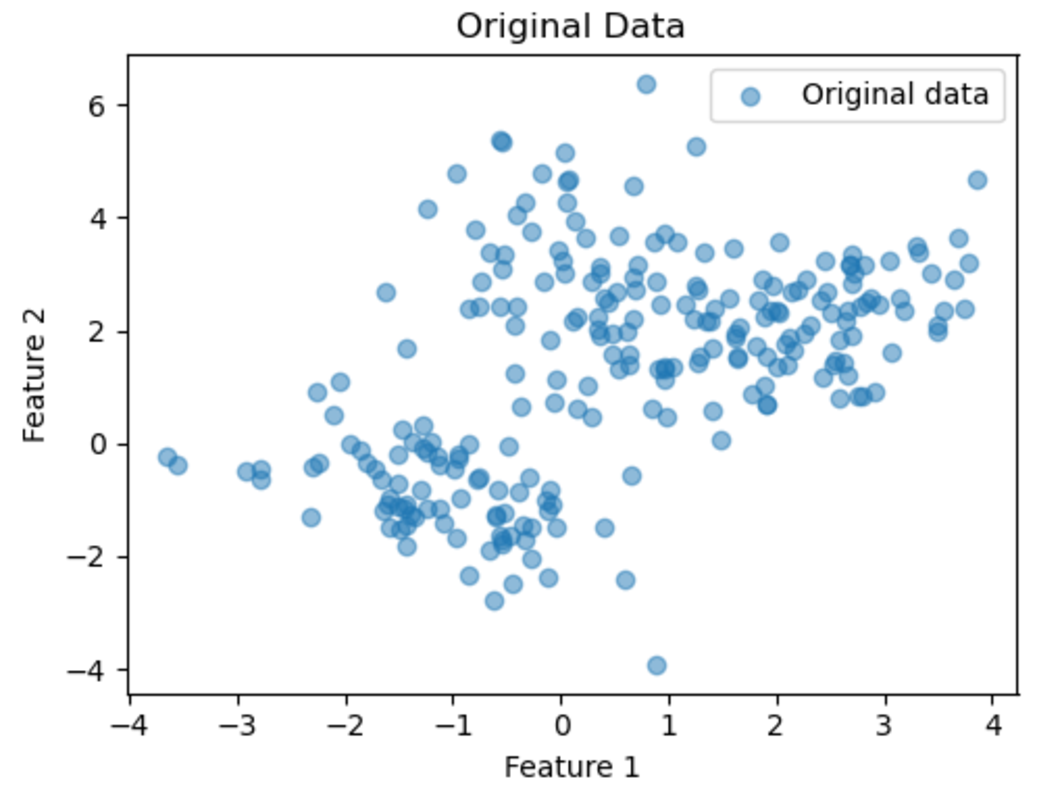
\includegraphics[scale=0.25]{./figs/original_data.pdf}&
      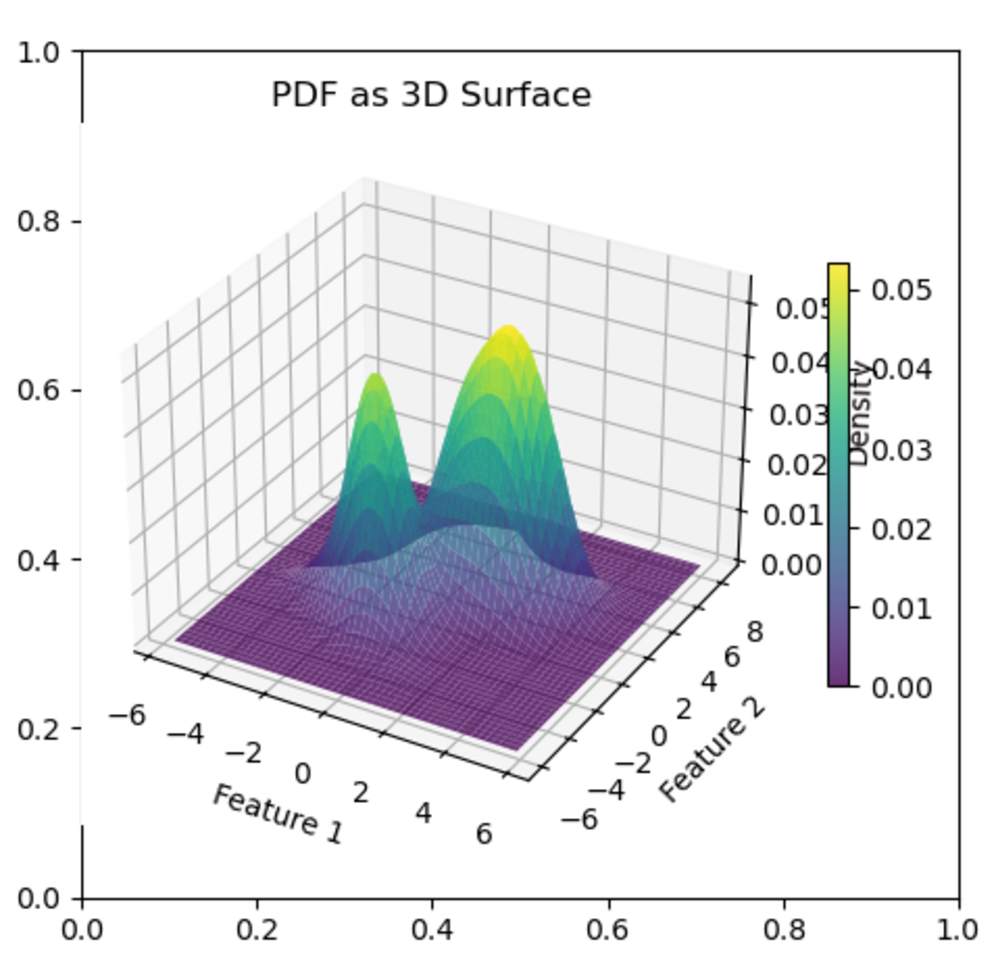
\includegraphics[scale=0.25]{./figs/PDF.pdf}
    \end{tabular}
  \end{center}
\end{frame}

\begin{frame}{From classification to generation}
\begin{itemize}
\item For classification tasks, we want to determine $P(y = k|\x)$ -
  the probability that a feature vector $\x$ belongs to class $k$.
  \vspace{0.5cm}
\item $p(\x) = \sum_{j=1}^K p(\x|y = j)P(y = j)$ is \alert{our main
  challenge} to estimate.
  \vspace{0.5cm}
\item The techniques could also be applied to $p(\x|y = k)$, if you
  use only samples from a class $k$.
  \vspace{0.5cm}
\item Knowledge of $p(\x)$ combined with labeled \textbf{representative} samples enables semi-supervised classification (pseudo-labeling) of unlabeled data.
\end{itemize}
We will be interested in using $p(\x)$ to \alert{generate} new representative
samples.
\end{frame}

\begin{frame}{Agenda}
  Goal: PDF estimation from \alert{finite data samples}, challenges,
  and applications.
  \vspace{0.5cm}
\begin{enumerate}
\item Non-parametric methods - make minimal assumptions about $p(\x)$.
  \vspace{0.5cm}
\item Parametric methods - Assume $p(\x)$ follows a known family (e.g., Gaussian).
  \vspace{0.5cm}
\item Manifolds and curse of dimensionality.  
  \vspace{0.5cm}
\item Applications: KL divergence, model comparison, and a real example.
\end{enumerate}
\end{frame}

\begin{frame}{Non-parametric PDF estimation}
For a dataset with $N$ samples, the methods usually rely on a region
$R$ of volume $V$ around each sample $\x$.

$$p(\x) = \lim_{V \to 0} \frac{\text{Number of points in region } R
  \text{ around } \x}{N\cdot V}$$
\vspace{0.5cm}
The region $R$ may be:
\begin{itemize}
\item A hypercube of side $h$ (\textbf{bandwidth}) and volume $V=h^n$.
\item A hypersphere of radius $h$ (\textbf{bandwidth}) and volume
$$ V={\frac {\pi ^{n/2}}{\Gamma {\bigl (}{\tfrac {n}{2}}+1{\bigr )}}}h^{n} $$ 
where $\Gamma$ is Euler's gamma function \alert{(preferred)}.
\end{itemize}
\end{frame}


\begin{frame}{Kernel-based methods}
An \alert{exponential kernel} is used around each sample $\x$ in both approaches:

$$\phi\left(\frac{\x_i-\x}{h}\right) = \exp\left(-\frac{\|\x_i-\x\|^2}{2h^2}\right)$$

The density estimate becomes:
$$p(\x) = \frac{1}{N\cdot V} \sum_{i \in S} \phi\left(\frac{\x_i-\x}{h}\right)$$

where $S$ is the set of samples to consider.

\begin{enumerate}
\item \textbf{Parzen Window:} $S = \{1, 2, \ldots, N\}$ (all samples), $V$ is fixed hypersphere volume  (see code1-parzen\_window.py). 
\item \textbf{k-NN:} $S = \{k \text{ nearest neighbors}\}$, $V$ adapts to contain exactly $k$ samples (see code2-knn\_density.py).
\end{enumerate}
\end{frame}

\begin{frame}{Curse of Dimensionality}
 Let $R$ be a hypersphere with radius $h=1$, its volume $V_n$ shrinks
 dramatically as the dimension $n$ increases.
\begin{itemize}
\item $n=2$: $V_2(1) = \pi \approx 3.14$ 
\item $n=5$: $V_5(1) \approx 5.26$ {\color{blue}← Peak}
\item $n=10$: $V_{10}(1) \approx 2.55$ {\color{orange}← Declining}
\item $n=20$: $V_{20}(1) \approx 0.026$ {\color{red}← Tiny!}
\item $n=100$: $V_{100}(1) \approx 10^{-40}$ {\color{red}← Negligible!}
\end{itemize}
Neighbors are \alert{far away} as $n$ increases, making the data
points \alert{isolated} and so the density estimates become
\alert{unreliable}. Conversely, to maintain unit volume, radius must
grow drastically (see code3-curse\_dimensionality.py).

\vspace{0.5cm} \pause

\begin{alertblock}{Bottom Line}
Parzen window and k-NN methods may fail for $n > 10$ dimensions.
\end{alertblock}

\end{frame}

\begin{frame}{Parametric PDF estimation}
Assuming that $p(\x)$ belongs to a known parametric family, the
\alert{problem} is to estimate its parameters $\btheta$ from the data
samples.

\vspace{0.5cm}

\textbf{Example:} A multivariate Gaussian distribution.

$$p(\x) = \mathcal{N}(\x|\bmu, \bSigma) =
\frac{1}{(2\pi)^{n/2}|\bSigma|^{1/2}}
\exp\left(-\frac{1}{2}(\x-\bmu)^T\bSigma^{-1}(\x-\bmu)\right)$$

where $\x, \bmu \in \mathbb{R}^n$ and $\bSigma \in \mathbb{R}^{n
  \times n}$ is positive definite (i.e., $\x^T \bSigma \x > 0$).

\vspace{0.5cm}

\textbf{Parameters $\btheta$:}
\begin{itemize}
\item $\bmu = (\mu_1, \ldots, \mu_n)^T$: mean vector.
\item $\bSigma$: $n \times n$ covariance matrix.
\end{itemize}

\end{frame}

\begin{frame}{Parameter estimation by maximum likelihood}
Given $N$ data samples $\{\x_1, \ldots, \x_N\}$, the maximum
likelihood estimates
\begin{align}
\hat{\bmu}    &= \frac{1}{N}\sum_{i=1}^N \x_i \nonumber \\
\hat{\bSigma} &= \frac{1}{N}\sum_{i=1}^N (\x_i - \hat{\bmu})(\x_i - \hat{\bmu})^T
\nonumber
\end{align}
\end{frame}

\begin{frame}{Whitening Transform: Data decorrelation}
  For $\x \sim \mathcal{N}(\bmu, \bSigma)$, let 
  \begin{itemize}
  \item $\mathbf{Q}$ be the \alert{eigenvectors} of
    $\bSigma=\mathbf{Q}\boldsymbol{\Lambda}\mathbf{Q}^T$, which define
    the principal axes of the data distribution, and
  \item $\boldsymbol{\Lambda} = \text{diag}(\lambda_1, \ldots,
    \lambda_n)$ be its \alert{eigenvalues} that define spread.
  \end{itemize}

\pause The \alert{whitening transform} defines the latent

$$\z = \bSigma^{-1/2}(\x - \bmu) \sim \mathcal{N}(\mathbf{0},
\mathbf{I}) $$

where

$$\bSigma^{-1/2} = \mathbf{Q}\boldsymbol{\Lambda}^{-1/2}\mathbf{Q}^T$$
$$\boldsymbol{\Lambda}^{-1/2} = \text{diag}(1/\sqrt{\lambda_1}, \ldots, 1/\sqrt{\lambda_n})$$
$$p(\z) = \frac{1}{(2\pi)^{n/2}} \exp\left(-\frac{1}{2}\|\z\|^2\right)$$

\textbf{Applications:} Generative models and dimensionality reduction. See code4-whitening\_transform.py and code5-gaussian\_analysis.py.

\end{frame}

\begin{frame}{Other computational simplification}
Many generative models (VAEs, normalizing flows) assume
\alert{diagonal covariance} for computational efficiency, sometimes
applying implicit whitening.

$$\bSigma = \text{diag}(\sigma_1^2, \ldots, \sigma_n^2)$$

\textbf{Simplified Gaussian with \alert{independent variables}:}

$$p(\x)=p(x_1)p(x_2)\ldots p(x_n)$$

$$p(\x) = \prod_{i=1}^n \frac{1}{\sqrt{2\pi\sigma_i^2}} \exp\left(-\frac{(x_i-\mu_i)^2}{2\sigma_i^2}\right)$$

\pause

\begin{alertblock}{Computational simplification:}
This simplification reduces from $\frac{n(n+1)}{2}$ parameters in the
full covariance to $n$ parameters in the diagonal one.
\end{alertblock}

\end{frame}

\begin{frame}{Mixture of Gaussians}
Real data often exhibits multiple clusters/modes (components).

\vspace{0.5cm}

\textbf{Solution:} Mixture of Gaussians (MoG)
$$p(\x) = \sum_{k=1}^K \pi_k \mathcal{N}(\x|\bmu_k, \bSigma_k)$$

where:
\begin{itemize}
\item $K$ is the number of components.
\item $\pi_k \geq 0$ are mixing weights with $\sum_{k=1}^K \pi_k = 1$.
\item $\mathcal{N}(\x|\bmu_k, \bSigma_k)$ is the $k$-th component.
\end{itemize}

\pause

\textbf{Parameters to estimate:}
$$\btheta = \{\pi_1, \ldots, \pi_K, \bmu_1, \ldots, \bmu_K, \bSigma_1, \ldots, \bSigma_K\}$$

\pause

\alert{How do we estimate $\btheta$?}

\end{frame}

\begin{frame}{KL Divergence: log-likelihood maximization}
  A PDF defined for the data samples only is
  $$p_{data}(\x) = \frac{1}{N}\sum_{i=1}^N \delta(\x - \x_i)$$ where
  $\delta$ is the Kronecker's delta. The KL divergence:
    
  $$D_{KL}(p_{data}(\x)||p(\x;\btheta)) = \int_{\mathbb{R}^n} p_{data}(\x) \log \frac{p_{data}(\x)}{p(\x;\btheta)} d\x$$

  $$ = \int_{\mathbb{R}^n} p_{data}(\x) \log p_{data}(\x) d\x - \int_{\mathbb{R}^n} p_{data}(\x) \log p(\x;\btheta) d\x$$

  $$ = C - \frac{1}{N} \int_{\mathbb{R}^n} \sum_{i=1}^N \delta(\x - \x_i)\log p(\x;\btheta) d\x = C - \frac{1}{N} \sum_{i=1}^N \log p(\x_i;\btheta)$$

  where the term $\ell(\btheta)=\sum_{i=1}^N \log p(\x_i;\btheta)$ is
  the \alert{log-likelihood}.
\end{frame}

\begin{frame}{KL Divergence: log-likelihood maximization}
  Since $p(\x;\btheta) = \sum_{k=1}^K \pi_k \mathcal{N}(\x|\bmu_k, \bSigma_k)$, direct maximum likelihood estimation is intractable due to sum inside
  logarithm
  
  $$\ell(\btheta) = \sum_{i=1}^N \log\left(\sum_{k=1}^K \pi_k \mathcal{N}(\x_i|\bmu_k, \bSigma_k)\right)$$.

  However, minimizing KL divergence is equivalent to maximizing $\ell(\btheta)$.
  
  $$\min_{\boldsymbol{\theta}} D_{KL}(p_{data}(\x)||p(\x;\boldsymbol{\theta})) \equiv \max_{\boldsymbol{\theta}} \sum_{i=1}^N \log p(\mathbf{x}_i;\boldsymbol{\theta})$$

  See code6-kl\_divergence.py
  
\end{frame}

\begin{frame}{Expectation-Maximization Algorithm}
\textbf{Key idea:} Introduce latent variables $z_{ik} \in \{0,1\}$
\begin{itemize}
\item $z_{ik} = 1$ if $\x_i$ belongs to component $k$, 0 otherwise
\item Only one $z_{ik} = 1$ per data sample $\x_i$
\end{itemize}

\pause 

\begin{block}{Complete data log-likelihood}
$$\ell_c(\btheta) = \sum_{i=1}^N \sum_{k=1}^K z_{ik}[\log \pi_k + \log \mathcal{N}(\x_i|\bmu_k, \bSigma_k)]$$
\end{block}

\pause

\textbf{EM Algorithm alternates:}
\begin{enumerate}
\item \textbf{E-step:} Compute $\gamma_{ik}^{(t)} = E[z_{ik}|\x_i, \btheta^{(t)}] = P(z_{ik}=1|\x_i, \btheta^{(t)})$
\item \textbf{M-step:} Maximize $E[\ell_c(\btheta^{(t)})]$ w.r.t. $\btheta^{(t)}$
\end{enumerate}

\pause

\textbf{Guaranteed:} Monotonic increase in likelihood until convergence
\end{frame}

\begin{frame}{EM Algorithm from $\btheta^{(0)} = \{\pi_k^{(0)}, \bmu_k^{(0)}, \bSigma_k^{(0)}\}$}
\begin{algorithmic}[1]
\REPEAT
\STATE \textbf{E-step:} For each $i, k$:
$$\gamma_{ik}^{(t+1)} = \frac{\pi_k^{(t)} \mathcal{N}(\x_i|\bmu_k^{(t)}, \bSigma_k^{(t)})}{\sum_{j=1}^K \pi_j^{(t)} \mathcal{N}(\x_i|\bmu_j^{(t)}, \bSigma_j^{(t)})}$$
\STATE \textbf{M-step:} Update parameters:
$$N_k^{(t+1)} = \sum_{i=1}^N \gamma_{ik}^{(t+1)}$$
$$ \pi_k^{(t+1)} = \frac{N_k^{(t+1)}}{N}, \quad \bmu_k^{(t+1)} = \frac{1}{N_k^{(t+1)}} \sum_{i=1}^N \gamma_{ik}^{(t+1)} \x_i$$
$$\bSigma_k^{(t+1)} = \frac{1}{N_k^{(t+1)}} \sum_{i=1}^N \gamma_{ik}^{(t+1)} (\x_i - \bmu_k^{(t+1)})(\x_i - \bmu_k^{(t+1)})^T$$
\STATE $t \leftarrow t + 1$
\UNTIL $|\ell_c(\btheta^{(t+1)})-\ell_c(\btheta^{(t)})| < \epsilon$.
\end{algorithmic}
\end{frame}

\begin{frame}{Model Selection: AIC and BIC}
\textbf{Problem:} How many components $K$ should we use in GMM?
\begin{itemize}
\item Too few $\rightarrow$ \alert{underfitting} (high bias)
\item Too many $\rightarrow$ \alert{overfitting} (high variance)
\end{itemize}
\vspace{0.3cm}\pause

\textbf{Solution:} Information criteria balance fit vs. complexity
\begin{block}{Akaike Information Criterion (AIC)}
$$\text{AIC}(K) = -2\ell(\btheta) + 2r$$
\end{block}
\begin{block}{Bayesian Information Criterion (BIC)}
$$\text{BIC}(K) = -2\ell(\btheta) + r \log N$$
\end{block}
where $r$ is the number of parameters.
\pause

\textbf{Strategy:} Choose $K$ that \alert{minimizes} AIC or BIC (code7-em\_algorithm.py).
\end{frame}

\begin{frame}{Real-world example}
  Let a store dataset with regular, premium, and occasional customers
  to study their behavior.
\vspace{0.5cm}\\
\begin{block}{Customer vectors $\x = (x_1, x_2) \in \mathbb{R}^2$}
    \vspace{0.5cm}
  \begin{itemize}
  \item $x_1$: Monthly spending (\$).
    \vspace{0.5cm}
  \item $x_2$: Visit frequency (visits/month).
  \end{itemize}
  \end{block}
  \vspace{1cm}
  \textbf{File:} \texttt{code8-customer\_analysis.py}
  
\end{frame}

\begin{frame}{Preview of the next lecture}
Real-world data often lives in high-dimensional spaces ($n \gg 10$) where:
\vspace{0.3cm}
\begin{itemize}
\item Direct visualization is impossible.
\vspace{0.5cm}
\item Traditional density estimation fails.
\vspace{0.5cm}
\item We need \alert{dimensionality reduction} techniques.
\end{itemize}
\vspace{0.3cm}\pause
\begin{block}{Fundamental questions}
\begin{itemize}
\item How can we visualize PDFs in $\mathbb{R}^{100+}$?
\vspace{0.5cm}
\item What is the intrinsic dimensionality of real data?
\vspace{0.5cm}
\item How do we preserve PDF structure when reducing dimension?
\end{itemize}
\end{block}
\end{frame}

\end{document}
